
\begin{figure}
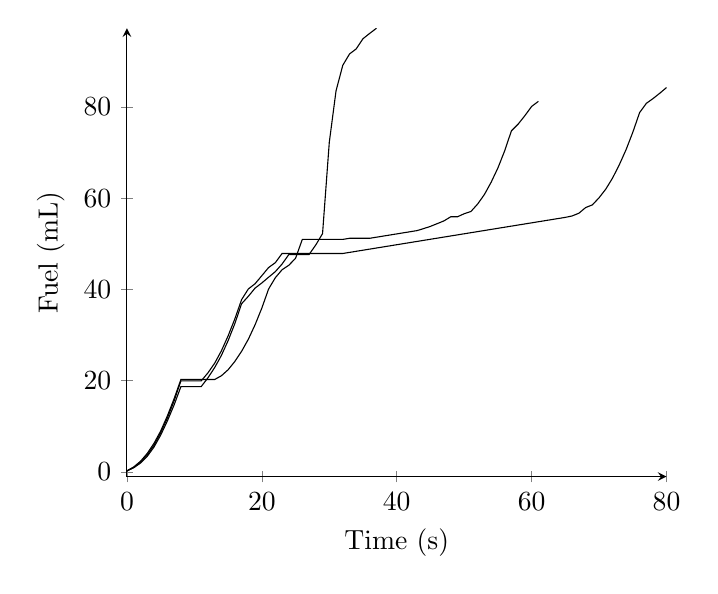
\begin{tikzpicture}
\begin{axis}[
legend style={anchor=west},
axis x line=bottom,
axis y line=left,
ymin=-1,
xlabel=Time (s),
ylabel=Fuel (mL),
]
\addplot[] coordinates {
(0, 0.239885513361)
(1, 0.923055400849)
(2, 1.94263359747)
(3, 3.40351794269)
(4, 5.4383190894)
(5, 8.06537952331)
(6, 11.1928491229)
(7, 14.7171513687)
(8, 18.7000814341)
(9, 18.7000814341)
(10, 18.7000814341)
(11, 18.7000814341)
(12, 20.6147836447)
(13, 22.8636436803)
(14, 25.5297718989)
(15, 28.7787623116)
(16, 32.5259766509)
(17, 36.8791485038)
(18, 38.5046650125)
(19, 40.3031893745)
(20, 41.4281414548)
(21, 42.6820643215)
(22, 43.9075881934)
(23, 45.5733193214)
(24, 47.6560137463)
(25, 47.6560137463)
(26, 47.6560137463)
(27, 47.6560137463)
(28, 49.7646452906)
(29, 52.2341437657)
(30, 72.2474815347)
(31, 83.5334688564)
(32, 89.1323770512)
(33, 91.6130972475)
(34, 92.7400092018)
(35, 94.9616765817)
(36, 96.1384636385)
(37, 97.258367572)
};
\addplot[] coordinates {
(0, 0.239885513361)
(1, 0.977158262565)
(2, 2.12416315903)
(3, 3.69402625372)
(4, 5.84329440117)
(5, 8.58611604014)
(6, 11.8341229145)
(7, 15.5882230921)
(8, 19.9547230428)
(9, 19.9547230428)
(10, 19.9547230428)
(11, 19.9547230428)
(12, 21.699356013)
(13, 23.8240698479)
(14, 26.5407780235)
(15, 29.8315041849)
(16, 33.5625730483)
(17, 37.7747466285)
(18, 40.1159786824)
(19, 41.2574838894)
(20, 43.0254731809)
(21, 44.8028494107)
(22, 45.8744696379)
(23, 47.8887375741)
(24, 47.8887375741)
(25, 47.8887375741)
(26, 47.8887375741)
(27, 47.8887375741)
(28, 47.8887375741)
(29, 47.8887375741)
(30, 47.8887375741)
(31, 47.8887375741)
(32, 47.8887375741)
(33, 48.1286230875)
(34, 48.3685086008)
(35, 48.6083941142)
(36, 48.8482796276)
(37, 49.0881651409)
(38, 49.3280506543)
(39, 49.5679361676)
(40, 49.807821681)
(41, 50.0477071944)
(42, 50.2875927077)
(43, 50.5274782211)
(44, 50.7673637344)
(45, 51.0072492478)
(46, 51.2471347612)
(47, 51.4870202745)
(48, 51.7269057879)
(49, 51.9667913013)
(50, 52.2066768146)
(51, 52.446562328)
(52, 52.6864478413)
(53, 52.9263333547)
(54, 53.1662188681)
(55, 53.4061043814)
(56, 53.6459898948)
(57, 53.8858754081)
(58, 54.1257609215)
(59, 54.3656464349)
(60, 54.6055319482)
(61, 54.8454174616)
(62, 55.085302975)
(63, 55.3251884883)
(64, 55.5650740017)
(65, 55.804959515)
(66, 56.1136102458)
(67, 56.7117343187)
(68, 57.9488912741)
(69, 58.5370856563)
(70, 60.1121325491)
(71, 62.0183318699)
(72, 64.4319983467)
(73, 67.349052446)
(74, 70.651233572)
(75, 74.4733817252)
(76, 78.7511226106)
(77, 80.7884894594)
(78, 81.8462185051)
(79, 83.0192791258)
(80, 84.2603280107)
};
\addplot[] coordinates {
(0, 0.239885513361)
(1, 1.09554148318)
(2, 2.326124685)
(3, 4.04768817492)
(4, 6.24064315058)
(5, 8.96581778224)
(6, 12.3089524988)
(7, 16.0831773092)
(8, 20.2641683409)
(9, 20.2641683409)
(10, 20.2641683409)
(11, 20.2641683409)
(12, 20.2641683409)
(13, 20.2641683409)
(14, 21.0836761473)
(15, 22.4053386526)
(16, 24.2281618474)
(17, 26.4456656193)
(18, 29.0984465508)
(19, 32.2686879263)
(20, 35.9250700166)
(21, 40.0948382291)
(22, 42.5788240359)
(23, 44.3242145192)
(24, 45.3044837389)
(25, 46.8426149483)
(26, 50.9682604177)
(27, 50.9682604177)
(28, 50.9682604177)
(29, 50.9682604177)
(30, 50.9682604177)
(31, 50.9682604177)
(32, 50.9682604177)
(33, 51.2211191445)
(34, 51.2211191445)
(35, 51.2211191445)
(36, 51.2211191445)
(37, 51.4610046579)
(38, 51.7008901712)
(39, 51.9407756846)
(40, 52.180661198)
(41, 52.4205467113)
(42, 52.6604322247)
(43, 52.9003177381)
(44, 53.3473648264)
(45, 53.8333122943)
(46, 54.4272930818)
(47, 55.0319216598)
(48, 55.9283130528)
(49, 55.9283130528)
(50, 56.6013976426)
(51, 57.0964136292)
(52, 58.7376288759)
(53, 60.822881059)
(54, 63.5125917214)
(55, 66.6409318126)
(56, 70.3854232042)
(57, 74.7758209165)
(58, 76.2457311511)
(59, 78.1044824078)
(60, 80.1179496159)
(61, 81.2331287232)
};

\end{axis}
\end{tikzpicture}
\label{tik:fuel:0:54}
\caption{0 percent diving with GSC on route $54$}
\end{figure}
